% Copyright 2004 by Till Tantau <tantau@users.sourceforge.net>.
%
% In principle, this file can be redistributed and/or modified under
% the terms of the GNU Public License, version 2.
%
% However, this file is supposed to be a template to be modified
% for your own needs. For this reason, if you use this file as a
% template and not specifically distribute it as part of a another
% package/program, I grant the extra permission to freely copy and
% modify this file as you see fit and even to delete this copyright
% notice. 

\documentclass[xcolor=table,aspectratio=169]{beamer}
\usepackage{menukeys}[os=win]
\usepackage{textcomp}
\usepackage{tcolorbox}
\usepackage{lmodern}
\usepackage{listings}
\lstset{
  basicstyle=\tiny\ttfamily,
}

% There are many different themes available for Beamer. A comprehensive
% list with examples is given here:
% http://deic.uab.es/~iblanes/beamer_gallery/index_by_theme.html
% You can uncomment the themes below if you would like to use a different
% one:
%\usetheme{AnnArbor}
%\usetheme{Antibes}
%\usetheme{Bergen}
%\usetheme{Berkeley}
%\usetheme{Berlin}
%\usetheme{Boadilla}
%\usetheme{boxes}
%\usetheme{CambridgeUS}
%\usetheme{Copenhagen}
%\usetheme{Darmstadt}
%\usetheme{default}
%\usetheme{Frankfurt}
%\usetheme{Goettingen}
%\usetheme{Hannover}
%\usetheme{Ilmenau}
\usetheme{JuanLesPins}
%\usetheme{Luebeck}
%\usetheme{Madrid}
%\usetheme{Malmoe}
%\usetheme{Marburg}
%\usetheme{Montpellier}
%\usetheme{PaloAlto}
%\usetheme{Pittsburgh}
%\usetheme{Rochester}
%\usetheme{Singapore}
%\usetheme{Szeged}
%\usetheme{Warsaw}
\setbeamerfont{block body}{size=\small}
\title{KF5004 - Primary \texttt{DNS} Server}
\titlegraphic{
\includegraphics[width=0.3\textwidth]{../images/logo.png}}

% A subtitle is optional and this may be deleted
% \subtitle{(Using proximity detection)}

\author{Dr.~Neil~Eliot \& Dr.~Alun~Moon}
% - Give the names in the same order as the appear in the paper.
% - Use the \inst{?} command only if the authors have different
%   affiliation.

%\renewcommand\appendixname{Appendix}

\institute[Northumbria University] % (optional, but mostly needed)
{
  Department of Computer and Information Sciences\\
  University of Northumbria
  % \and
  % \inst{2}
  % Department of Theoretical Philosophy\\
  % University of Elsewhere
}
% - Use the \inst command only if there are several affiliations.
% - Keep it simple, no one is interested in your street address.

\date{Session 5}
% - Either use conference name or its abbreviation.
% - Not really informative to the audience, more for people (including
%   yourself) who are reading the slides online

\subject{Introduction}
% This is only inserted into the PDF information catalog. Can be left
% out. 

% If you have a file called "university-logo-filename.xxx", where xxx
% is a graphic format that can be processed by latex or pdflatex,
% resp., then you can add a logo as follows:

% \pgfdeclareimage[height=0.5cm]{university-logo}{university-logo-filename}
% \logo{\pgfuseimage{university-logo}}

% Delete this, if you do not want the table of contents to pop up at
% the beginning of each subsection:
% \AtBeginSubsection[]
% {
%   \begin{frame}<beamer>{Outline}
%     \tableofcontents[currentsection,currentsubsection]
%   \end{frame}
% }

% Let's get started

\begin{document}

\begin{frame}
  \titlepage
\end{frame}

\begin{frame}{Introduction}
  \tableofcontents
  % You might wish to add the option [pausesections]
\end{frame}

% Section and subsections will appear in the presentation overview
% and table of contents.

\section{Introduction}
\subsection{\texttt{rDNS}}
\begin{frame}{\texttt{rDNS} Reverse Mapping}
  \begin{itemize}
    \item Given an \texttt{IP} address \texttt{DNS} can determine the host name.
    \item Although sometimes this is required for diagnostic purposes, more frequently these days it is used for security reasons to trace a hacker or spammer.
      \begin{itemize}
        \item It confirms that the \texttt{IP} address contained in the \texttt{IP} packet header of a mail message does represent the indicated host.
      \end{itemize}
    \item In order to perform reverse mapping \texttt{DNS} designers have defined a special (reserved) domain name.
    \begin{itemize}
      \item \texttt{in-addr.arpa.}
    \end{itemize}
\end{itemize}
\end{frame}

\begin{frame}{\texttt{DNS} Recap}
  \begin{itemize}
    \item Normal \texttt{domain name} structure is hierarchical, starting from the root (.).
    \item A \texttt{domain name} is written left to right, but the hierarchical structure is written right to left.
      \begin{itemize}
        \item \texttt{www.example.com.}
      \end{itemize}
  \end{itemize}
\end{frame}

\begin{frame}{\texttt{DNS} Recap}
  \begin{itemize}
    \item The highest node in the \texttt{DNS} hierarchy (or tree) is the root. Defined by the normally silent (omitted) dot. 
      \begin{itemize}
        \item e.g. \texttt{.}
      \end{itemize}
    \item This is followed by the Top-Level Domain (\texttt{TLD}). 
      \begin{itemize}
        \item e.g. \texttt{.com}
      \end{itemize}
    \item Next (lower) is the Second-Level \texttt{Domain}
      \begin{itemize}
        \item e.g. \texttt{.example}
      \end{itemize}
    \item Finally the lowest is the \texttt{host name}
      \begin{itemize}
        \item e.g. \texttt{www}
      \end{itemize}    
  \end{itemize}
  \begin{tcolorbox}
    \begin{center}
      \texttt{www.example.com.}      
    \end{center}
  \end{tcolorbox}
\end{frame}

\section{Mapping}
\subsection{\texttt{rDNS}}
\begin{frame}{How are addresses mapped?}
  \begin{itemize}
    \item The Internet \texttt{Domain names} are managed and controlled by \texttt{ICANN}.
      \begin{itemize}
        \item \texttt{I}nternet \texttt{C}orporation for \texttt{A}ssigned \texttt{N}ames and \texttt{N}umbers
      \end{itemize}
    \item Each \texttt{domain} contains \texttt{labels} separated by dots.
      \begin{itemize}
        \item The right-most label in a \texttt{domain name} is referred to as its "top-level domain" (\texttt{TLD}).
      \end{itemize}
    \item The \texttt{DNS} forms a tree-like hierarchy. 
      \begin{itemize}
        \item Each \texttt{TLD} includes many second-level domains (such as \texttt{icann} in \texttt{www.icann.org}); each second-level \texttt{domain} can include a number of third-level \texttt{domains} (\texttt{www} in \texttt{www.icann.org}), and so on.
      \end{itemize}
  \end{itemize}
\end{frame}

\begin{frame}{How are addresses mapped?}
  \begin{itemize}
    \item The responsibility for operating each \texttt{TLD} (including maintaining a registry of the second-level \texttt{domains} within the \texttt{TLD}) is delegated to a particular organization. 
      \begin{itemize}
        \item These organizations are referred to as `registry operators'.
        \item You register your \texttt{names} with these companies for them to be public.
      \end{itemize}
  \end{itemize}
\end{frame}

\begin{frame}{How are addresses mapped?}
  \begin{itemize}
    \item In the 1980s there were only seven \texttt{gTLD}s (\texttt{.com, .edu, .gov, .int, .mil, .net, and .org}) 
    \item \texttt{Domain names} could be registered in three of these (\texttt{.com, .net, and .org}) without restriction; the other four had restrictions.
    \item More domains have been released:
      \begin{itemize}
        \item \texttt{.co.uk}
        \item \texttt{.me}
        \item etc.
      \end{itemize}
  \end{itemize}
\end{frame}

\begin{frame}{How are addresses mapped?}
  \begin{itemize}
    \item Logical mapping. 
  \end{itemize}
  \begin{figure}
    \begin{center}
      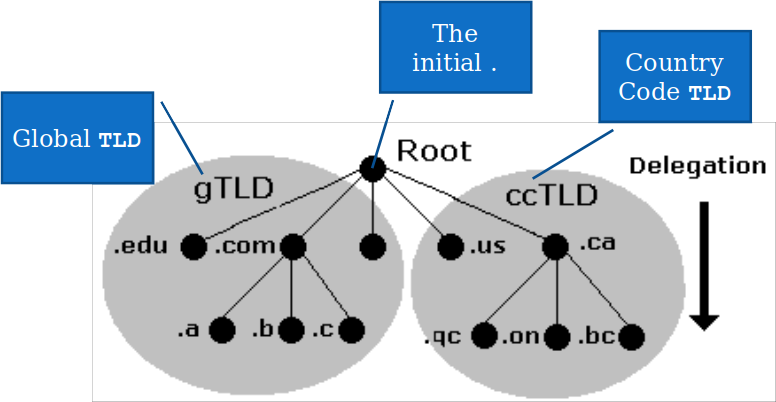
\includegraphics[width=0.6\linewidth]{DNS.png}
    \end{center}
  \end{figure}
\end{frame}

\subsection{\texttt{root hints}}
\begin{frame}{How are root addresses mapped?}
  \begin{itemize}
    \item \texttt{InterNIC} - Manage the public information regarding Internet Domain Name Registration Services. 
      \begin{itemize}
        \item \texttt{http://www.internic.net/zones/named.root} 
      \end{itemize}
    \item This file can be used by \texttt{primary} and \texttt{secondary} servers to use the \texttt{root servers} rather than \texttt{forwarders}.
      \begin{itemize}
        \item \texttt{/etc/bind/db.root} 
      \end{itemize}
    \item If you want your server to \texttt{root hints} this file should be updated \textbf{bi-monthly}.
  \end{itemize}
\end{frame}

\subsection{\texttt{rDNS} Domain}
\begin{frame}{\texttt{rDNS} background}
  \begin{itemize}
    \item An \texttt{IPv4} address is written:-
      \begin{itemize}
        \item \texttt{182.168.100.254/24} 
      \end{itemize}
    \item This \texttt{IPv4} address defines a \texttt{host} address of 254 in the \texttt{Class C} address range \texttt{192.168.100.x}
    \item In this case, the most important part (the highest node) is on the left (\texttt{192}), not the right. 
    \item This makes it impossible to construct a sensible tree structure that could be searched starting at the left most octet.
  \end{itemize}
\end{frame}

\begin{frame}{\texttt{rDNS} background}
  \begin{itemize}
    \item \texttt{rDNS} requires a different approach.
      \begin{itemize}
        \item Create the \texttt{domain name}, reverse the order of the address, build the hierarchy under the special \texttt{domain name}.
      \end{itemize}
    \item \texttt{in-addr.arpa.}
      \begin{itemize}
        \item \texttt{SLD} is \texttt{in-addr}
        \item \texttt{TLD} is \texttt{arpa}
      \end{itemize}
  \end{itemize}
\end{frame}

\begin{frame}{\texttt{rDNS} background}
  \begin{itemize}
    \item \texttt{DNS} and \texttt{rDNS} Delegation. 
  \end{itemize}
  \begin{figure}
    \begin{center}
      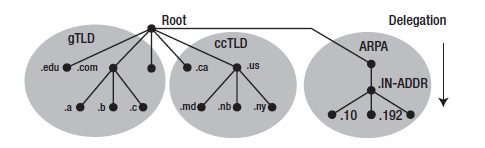
\includegraphics[width=1\linewidth]{Delegate.png}
    \end{center}
  \end{figure}
\end{frame}

\subsection{Implementation}
\begin{frame}[fragile]{Add the Reverse \texttt{zone}}
  \begin{itemize}
    \item Modify \texttt{named.conf.local}
  \end{itemize}
  \begin{tcolorbox}
    \lstset{
      basicstyle=\tiny\ttfamily,
    }
    \begin{lstlisting}
          zone "100.168.192.in-addr.arpa" {
            type master;
            notify no;
            file "/etc/bind/db.100.168.192.in-addr.arpa";
          };
    \end{lstlisting}
  \end{tcolorbox}
  \begin{tcolorbox}[title={\textbf{NOTE:}}]
    \begin{center}
      \scriptsize More on the filename in a moment.
    \end{center}
  \end{tcolorbox}
\end{frame}

\begin{frame}{\texttt{rDNS} background}
  \begin{itemize}
    \item \texttt{192.168.100.254/24} 
      \begin{itemize}
        \item \texttt{IPv4} address \texttt{254} is the \texttt{host address} defined in the \texttt{zone}.
      \end{itemize}
    \item The name is constructed as follows:
      \begin{itemize}
        \item \texttt{Class C}  base is \texttt{192.168.100}
        \item Reverse the base - \texttt{100.168.192}
        \item Add the \texttt{rDNS TLD} and \texttt{SLD}
      \end{itemize}
  \end{itemize}
  \begin{tcolorbox}
    \begin{center}
      The \texttt{rDNS domain} for \texttt{192.168.100.254/24} is \texttt{100.168.192.in-addr.arpa.} and the \texttt{host name} is \texttt{254}       
    \end{center}
  \end{tcolorbox}
\end{frame}

\begin{frame}{Resource Record (\texttt{RR}) for \texttt{rDNS}}
  \begin{itemize}
    \item Reverse mapping uses the \texttt{PTR} Resource Record.
    \item The \texttt{PTR RR} is standardized in \texttt{RFC 1035}
    \item Maps an \texttt{IPv4} and \texttt{IPv6} addresses to a particular host in the \texttt{domain}.
  \end{itemize}
\end{frame}

\begin{frame}{\texttt{PTR} - Resource Record (\texttt{RR}) for \texttt{rDNS}}
  \begin{itemize}
    \item Syntax.
      \begin{itemize}
        \item \texttt{name ttl class rr name}
      \end{itemize}
    \item e.g.
      \begin{itemize}
        \item \texttt{254     IN PTR ns.example.com.}
      \end{itemize}
  \end{itemize}
  \begin{tcolorbox}[title={\textbf{NOTE:}}]
    \begin{center}
      \scriptsize The terminating period (.) is very important.
    \end{center}
  \end{tcolorbox}
\end{frame}

\begin{frame}{\texttt{PTR}}
  \begin{table}
    \rowcolors{1}{}{lightgray} %-- this indicates the change in odd and pair rows
    \tiny
    \begin{tabular}{|p{1.6cm}|p{1.6cm}|p{4.7cm}|} 
      \hline
      \rowcolor{gray}
      \multicolumn{1}{|c|}{Syntax} & \multicolumn{1}{c|}{Example} & \multicolumn{1}{c|}{Description}\\ 
      \hline
      \texttt{name}&254&Although this looks like a number, it is in fact treated as a \texttt{name}. The \texttt{name} is unqualified, causing the \texttt{\$ORIGIN} directive value to be substituted. You could have written this as 254.100.168.192.INADDR.ARPA. (using the FQDN format).\\
      \hline
      \texttt{ttl}&&There is no \texttt{ttl} value defined for the \texttt{RR} (in this case), so the zone default of \texttt{2d} (172800 seconds) from the \texttt{\$TTL} directive will be used.\\
      \hline
      \texttt{class}&\texttt{IN}&\texttt{IN} defines the class to be Internet (defaulted if omitted). Other values exist but are rarely used.\\
      \hline
      \texttt{name}&\texttt{ns.example.com.}&Defines that a query for \texttt{192.168.100.254} will return \texttt{ns.example.com.} This name must be written in the \texttt{FQDN} notation \texttt{\$ORIGIN} would create the wrong name.\\
      \hline
    \end{tabular}
  \end{table}
\end{frame}

\begin{frame}{Create the \texttt{reverse zone} file}
  \begin{itemize}
    \item Create the new zone file from a template
  \end{itemize}
  \begin{tcolorbox}
    \begin{center}
      \texttt{\scriptsize\$sudo cp /etc/bind/db.127 /etc/bind/db.100.168.192.in-addr.arpa}
    \end{center}
  \end{tcolorbox}
  \begin{itemize}
    \item  Edit the new \texttt{db.100.168.192.in-addr.arpa} file changing the details in a similar way to the original \texttt{zone} file except you now add \texttt{PTR} records rather than \texttt{A} records.
  \end{itemize}
  \begin{tcolorbox}[title={\textbf{NOTE:}}]
    \begin{center}
      \scriptsize A \texttt{class B} address (\texttt{192.168.100.254/16}) would have a \texttt{reverse domain} of \texttt{168.192.in-addr.arpa}
    \end{center}
  \end{tcolorbox}
\end{frame}

\begin{frame}[fragile]{Create the \texttt{reverse zone} file}
  \begin{itemize}
    \item Original \texttt{db.127} file
  \end{itemize}
  \begin{tcolorbox}
    \lstset{
      basicstyle=\tiny\ttfamily,
    }
    \begin{lstlisting}
      ;
      ; BIND reverse data file for local loopback interface
      ;
      $TTL    604800
      @       IN      SOA     localhost. root.localhost. (
                                    1         ; Serial
                               604800         ; Refresh
                                86400         ; Retry
                              2419200         ; Expire
                               604800 )       ; Negative Cache TTL
      ;
      @       IN      NS      localhost.
      1.0.0   IN      PTR     localhost.
    \end{lstlisting}
  \end{tcolorbox}
\end{frame}

\begin{frame}[fragile]{Create the \texttt{reverse zone} file}
  \begin{itemize}
    \item New \texttt{db.100.168.192.in-addr.arpa} file
  \end{itemize}
  \begin{tcolorbox}
    \lstset{
      basicstyle=\tiny\ttfamily,
    }
    \begin{lstlisting}
      ;
      ; BIND reverse data file for local interface
      ;
      $TTL    604800
      $ORIGIN 100.168.192.in-addr.arpa.
      @       IN      SOA     ns.example.com. admin.example.com. (
                           2020010101         ; Serial
                               604800         ; Refresh
                                86400         ; Retry
                              2419200         ; Expire
                               604800 )       ; Negative Cache TTL
      ;
      @        IN      NS      ns.example.com.
      254      IN      PTR     ns.example.com.
          \end{lstlisting}
  \end{tcolorbox}
\end{frame}

\begin{frame}[fragile]{Create the \texttt{reverse zone} file}
  \begin{itemize}
    \item If the file was for a \texttt{Class C zone}
  \end{itemize}
  \begin{tcolorbox}
    \lstset{
      basicstyle=\tiny\ttfamily,
    }
    \begin{lstlisting}
      ;
      ; BIND reverse data file for local interface
      ;
      $TTL    604800
      $ORIGIN 168.192.in-addr.arpa.
      @       IN      SOA     ns.example.com. admin.example.com. (
                           2020010101         ; Serial
                               604800         ; Refresh
                                86400         ; Retry
                              2419200         ; Expire
                               604800 )       ; Negative Cache TTL
      ;
      @            IN      NS      ns.example.com.
      254.100      IN      PTR     ns.example.com.
          \end{lstlisting}
  \end{tcolorbox}
\end{frame}

\section{Security}
\subsection{General}
\begin{frame}{Create the \texttt{reverse zone} file}
  \begin{itemize}
    \item You should only set up \texttt{reverse zone} entries (\texttt{PTR} records) on services that need \texttt{rDNS} for authentication e.g. Mail Servers
  \end{itemize}
  \begin{tcolorbox}[title={\textbf{NOTE:}}]
       \scriptsize Setting up \texttt{rDNS} on all machines opens up the possibility of machines being used as spambots.
  \end{tcolorbox}
  \begin{tcolorbox}[title={\textbf{INFO:}}]
    \begin{center}
      \tiny{\texttt{https://www.mxpolice.com/email-security/importance-of-ptr-records-for-reliable-mail-delivery/}}      
    \end{center}
\end{tcolorbox}
\end{frame}

\subsection{Example}
\begin{frame}[fragile]{And Finally....}
  \begin{itemize}
    \item Using \texttt{rDNS}, the \texttt{MX IP} address of the `alleged' server \texttt{gmail.com} can be validated. 
  \end{itemize}
  \begin{tcolorbox}
    \lstset{
      basicstyle=\tiny\ttfamily,
    }
    \begin{lstlisting}
From: Media Temple user (user@gmail.com)
Subject: article: How to Trace a Email
Date: January 25, 2019 3:30:58 PM PDT
To: user@example.com
Return-Path: <user@gmail.com>
Envelope-To: user@example.com
Delivery-Date: Tue, 25 Jan 2011 15:31:01 -0700
Received: from po-out-1718.google.com ([72.14.252.155]:54907) 
by cl35.gs01.gridserver.com with esmtp (Exim 4.63) (envelope-from 
<user@gmail.com>) id 1KDoNH-0000f0-RL for user@example.com; Tue, 
25 Jan 2019 15:31:01 -0700
Received: by po-out-1718.google.com with SMTP id y22so795146pof.4
 for <user@example.com>; Tue, 25 Jan 2019 15:30:58 -0700 (PDT)
    \end{lstlisting}
  \end{tcolorbox}
\end{frame}

\section*{Conclusion}
\begin{frame}{Conclusion}
  \begin{itemize}
    \item What is the purpose of a \texttt{Reverse Lookup Zone}?
    \item How do you create a \texttt{rDNS} zone?
    \item What is an \texttt{PTR} record?
  \end{itemize}
\end{frame}

\end{document}


